\chapter{Introduction}
\label{sec:intro}

\section{Graphs Are Ubiquitous}
\label{sec:intro:ubiquitous}

New data are being generated rapidly, and there is an ever-present and growing need to store and analyze them efficiently.
Much of this data has some inherent schema or structure, and relational databases are a natural choice for efficient storage.
\ac{RDBMS} have been the backbone of data management for six decades and have been repeatedly extended to service new and emerging use cases \cite{stonebraker2018c,boncz2005monetdb, HStore2008Abadi, stonebraker2013voltdb,PASE2020:pgvector}.
RDBMSs are well-suited for storing and querying structured or semi-structured data on workloads with high volumes of small updates and stringent consistency requirements; these tasks are called \ac{OLTP} workloads.
Larger scale data analysis frequently requires full dataset scans and extensive join processing, and these data warehouse or \ac{BI} workloads are called \ac{OLAP}.
Several relational OLAP databases and data warehousing solutions exist to enable such enterprise-scale workloads~\cite{Redshift2015,boncz2005monetdb,vertica, raasveldt2019duckdb}.

However, in some applications, the relationships captured in the data are themselves a fundamentally important object of study. 
Graphs are a natural data model for relationships between entities in social networks, the World Wide Web, recommendation systems, fraud detection, and biological networks~\cite{ubiquityLargeGraphsVLDB2017}.
As the data volumes grow, so do the graphs these relationships form.
Applications now routinely store and analyze graphs with billions of nodes and trillions of edges~\cite{ching2015oneTrillion,besta2020demystifying, lin2018shentu, gupta2024graphscale, zhou2025redtao}.

These large graphs are now ubiquitous, and more than a decade of research has investigated how to store and process them efficiently.
Each vertex and edge in such a graph has a \emph{label} that assigns it a type (e.g., ``User,'' ``follows''), and may contain \emph{properties} modeled as key-value attributes (e.g., \texttt{name}, \texttt{age}).
Graphs in which the nodes have properties and the edges have labels are called Labeled Property Graphs~\cite{besta2020demystifying}.
The labels and properties give the graph \emph{semantic meaning}, while the nodes and edges alone form the \emph{structure} of the graph.

\section{Graph Workloads: OLTP vs.\ OLAP}
\label{sec:intro:workloads}

Graph workloads fall into categories analogous to conventional database workloads.
\ac{OLTP} queries on graphs resemble their tabular counterparts; for example, in a social network, a user might wish to see the latest posts and replies on their favorite ongoing Twitter feud~\cite{AholeMusk:online}.
Such \emph{interactive} queries are latency-sensitive, with many tasks, such as fraud detection in financial networks, demanding 20\,ms latencies~\cite{qiu2018real}.

Analytical workloads on graphs (graph \ac{OLAP}) are queries about the network that can be answered only through ``whole-graph'' analysis; they operate on the graph structure and typically ignore labels and properties.
For example, the recommendation teams at Twitter run PageRank and topic-similarity tasks on the user-follow graph to measure the influence of users and recommend new users to follow~\cite{tang2022taming}.
The health teams at Twitter and Facebook run multi-account and fake account detection algorithms on the network graphs to identify and remove fake accounts~\cite{breuer2020friend}.
These tasks interact with large parts of the graph, if not the whole graph, and take longer to finish.

These two workload classes are served by different systems: graph databases for OLTP and specialized graph processing systems for OLAP.
This dual-silo approach incurs substantial \ac{ETL} overhead and consistency challenges.\PM{insert citations and maybe 1 line discussion}

\section{Current Approaches and Their Limitations}
\label{sec:intro:approaches}

Graph analysis tasks typically access the whole graph, or a significant part of it.
If we store the graph only in its relational form, relations (edges) are encoded as joins, and graph traversals turn into recursive self-joins~\cite{10.1145/3129246}.
RDBMSs do not perform well for graph analytics tasks, because computing these recursive self-joins is expensive and their cost grows with path length~\cite{TransitiveClosureBiskupStiefeling1989}.

Substantial effort has gone into enabling graph analytics within databases.
One line of work stores graphs in relational tables and routes analytics to a separate in-memory engine: Facebook's TAO~\cite{bronson2013tao} serves the social graph from MySQL but delegates analytics to offline pipelines; Oracle loads property graphs into PGX, an in-memory graph server, for analysis~\cite{OraclePG,WhatIsOracleSpatialGraph:online,hong2015pgx,welc2013graph,hong2013early}.
A complementary line extends SQL with graph syntax, most notably SQL/Property Graph Query Language (SQL/PGQL)~\cite{duckpgq:online}, but these extensions build only transient in-memory representations and lack persistent graph layouts or transactional mutation support.
None of these approaches provides a single persistent store with analytics-friendly layouts and integrated transactional mutation.

In response to this mismatch, we have witnessed an explosion in special-purpose systems for storing and processing graph-structured data.
Specialized graph databases such as Neo4j~\cite{neo4j} and ArangoDB~\cite{arangodb} follow in the tradition of relational databases, providing a schema-oriented organization and a high-level query language.
These systems work well for OLTP workloads but frequently exhibit suboptimal performance on OLAP tasks.
Neo4j, for instance, stores all graph data on disk as ``linked lists of fixed size records''~\cite{neo4j:data_layout:2024}.
A linked-list representation is effective for connectivity queries but causes catastrophic random access overhead when running whole-graph analytics.

In contrast, graph processing systems such as Pregel~\cite{malewicz2010pregel}, GraphX~\cite{gonzalez2014graphx}, PowerLyra~\cite{powerlyra2019}, GraphChi ~\cite{kyrola2012graphchi}, and Ligra~\cite{shun2013ligra} deliver outstanding OLAP performance but do not provide OLTP-style query capabilities.
Using them requires extracting the structural graph from the database, transforming it for ingestion, and loading it; a costly ETL pipeline.

\textit{This is the central dichotomy of graph data management}: graph databases provide \emph{persistent graph storage} but are outperformed on OLAP by specialized processing systems, which need a costly ingest and preprocessing phase before analytics can begin.
This split system design leads to a freshness mismatch between the data in the primary store, the data available for point queries in the graph database, and the data available for batch analysis in the graph processing system.

\section{Hybrid Systems (HGTAP)}
\label{sec:intro:hgtap}

The dichotomy described above has an equivalent in the relational database world: the constant data transformation needed to maintain consistency between a row-store and a column store~\cite{HTAP2016ArchepelagoArulraj}.
The development of \ac{HTAP} databases is a promising solution for relational workloads, and similar solutions must be developed for graph data management.

This motivated the development of Hybrid Graph Transactional and Analytical Processing (\ac{HGTAP}) systems, such as LiveGraph~\cite{zhu2019livegraph} and GART~\cite{shen2023bridging}.
LiveGraph stores adjacency lists in a large memory-mapped region (considered harmful~\cite{crotty2022you}) and its analytics-friendly layout delivers robust OLAP performance.
However, its transaction manager serializes writers, limiting insertion throughput~\cite{libinzhou2025GTX}.
GART constructs an in-memory multi-versioned \ac{CSR} bounded by main-memory capacity.
GART has been designed for latency and freshness-sensitive tasks, such as fraud detection, and not for the downstream batch processing tasks we target.
A practical graph data management system must support high-throughput ingestion and mutation, whole-graph analytics, and transactional property graph queries, and it must do so whether the graph fits in memory or exceeds it.
Neither LiveGraph nor GART meets all of these requirements.

\section{Key Observations}
\label{sec:intro:observations}

State-of-the-art systems typically assume that graph databases and graph processing systems run on a distributed collection of nodes.
We start with a different assumption: the best distributed system is built from the best single-node system.
Past research supports this position.
McSherry et al. introduced the COST metric (Configuration that Outperforms a Single Thread)~\cite{mcsherry2015scalability} and demonstrated that several popular distributed graph processing systems evaluated their scalability by comparing against poor single-threaded baselines rather than against efficient sequential implementations.
When McSherry compared these systems to an efficient sequential implementation, some could not match ``laptop performance'' regardless of how many machines were used.
This result led to benchmark standardization efforts~\cite{capotua2015graphalytics,mehrotra2024sok,beamer2015gap,graph500}, each identifying the need for more performant baseline algorithms and more comprehensive performance metrics.
Distributed graph processing is fundamentally inefficient due to communication costs~\cite{beamer2016understanding}; the main benefit of a cluster is aggregate RAM sufficient to keep the graph in memory.
The Waterloo survey on the state of graph processing~\cite{ubiquityLargeGraphsVLDB2017} reports that several respondents operate on uncompressed graphs larger than 1\,TB, but as we and others have shown, semi-external processing\footnote{In semi-external systems, vertex and algorithmic state is maintained in RAM and the graph edges are read from the storage device.} on a single node with fast storage can match or exceed distributed performance.
We design and optimize a single-node, single-socket graph database before requiring distribution.

Based on our study of the graph data management landscape, we make five observations:
\begin{enumerate}
  \item \textit{Layout construction time is non-trivial.} A significant amount of time in graph analytics is spent building the in-memory or on-disk data layout, not running the algorithm. Creating these layouts requires preprocessing the graph, a significant overhead relative to the cost of running many computations. Preprocessing costs are rarely amortized.
  \item \textit{Transaction management is expensive to build from scratch.} Dynamic graphs require ACID transactions, crash recovery, and concurrency control; substantial engineering that every new system must reimplement.
  \item \textit{No single operating regime suffices.} In-memory systems cannot handle graphs that exceed RAM; out-of-core systems sacrifice speed; distributed processing suffers from severe communication overhead~\cite{mcsherry2015scalability,beamer2016understanding} and poor work balance~\cite{hajidehi2023cuttana}. A practical system must span in-memory and out-of-core regimes.
  \item \textit{Data layout is the key determinant of performance.} An analytics-friendly persistent layout that preserves scan locality can serve both OLTP and OLAP workloads and can be extended to store full property graphs with typed, columnar storage.
  \item \textit{Most existing systems target a single operating point}: in-memory or out-of-core processing, static or dynamic graphs, structural or property graphs. Few perform well across the entire spectrum.
\end{enumerate}

\section{\project{}: Our Approach}
\label{sec:intro:flexograph}

This thesis presents the design of \project{}, a flexible and performant \ac{HGTAP} database system.
\project{} has been designed for a single-node setting and provides a fully transactional \ac{API} for updating and querying a graph.
Rather than building a custom storage engine, \project{} is built on the \wt{}~\cite{WiredTigerDocumentation} key-value store, inheriting a mature transaction manager, write-ahead log, and buffer pool at no additional engineering cost.

\project{} encodes two analytics-friendly structural layouts (adjacency lists and a CSR approximation) as sorted key ranges in \wt{}, producing sequential scan performance for analytics.
It extends these layouts with a typed property storage layer supporting both embedded and columnar modes.
\project{} eliminates the preprocessing step that other systems require before running analytics; its persistent layouts are ready for analysis at all times.
Insertion throughput scales near-linearly to 72 threads, sustaining up to 1.48\,M edges/sec on the write-optimized layout (\autoref{fig:dynamic-scaling}), while property-mutation latencies are three to four orders of magnitude lower than Neo4j~\cite{neo4j} and JanusGraph~\cite{janusgraph}.

A programmer uses \project{} through a library API that exposes read-only snapshot iterators over neighborhoods and properties to express analytics tasks.
The API is flexible enough to let users write algorithms as vertex or edge programs.
We modified the \ac{GAPBS}~\cite{beamer2015gap} to use this API and show that \project{}'s end-to-end analytics performance matches in-memory systems while scaling to out-of-core graphs.
We also evaluate the benefits of storing the graph's structure independently from its properties and contrast it with the choice to store them together.

\autoref{fig:fg-spider} summarizes these results: \project{} delivers robust performance across the entire spectrum of operating conditions, where every other system we evaluate falters significantly in two or more regimes.
A system purpose-built for a single regime can outperform \project{} in that niche; Teseo significantly outperforms us on dynamic graph ingest and update operations.
No other system we evaluate matches its breadth while providing full transactional guarantees.

Our contributions are as follows.
\begin{itemize}
  \item The design of \project{}, a hybrid graph database built on \wt{} that unifies OLTP and OLAP graph workloads in a single persistent store without ETL or preprocessing.
  \item An analysis of analytics-friendly data layouts and a demonstration of how adjacency-list and CSR-like representations can be encoded as sorted key ranges in a key-value store to preserve scan locality.
  \item A typed property storage layer with embedded and columnar modes that achieves property-mutation latencies three to four orders of magnitude lower than that of Neo4j, JanusGraph, and ArangoDB.
  \item Efficient, read-only neighborhood iterators on graph snapshots, with a flexible partitioning strategy that splits work between threads by vertex count or edge count.
  \item An evaluation showing that \project{} matches the analytics performance of in-memory and out-of-core graph processing systems, scales insertion throughput near-linearly, and delivers the transactional performance of in-memory dynamic graph containers.
\end{itemize}

\begin{figure}[t]
  \centering
  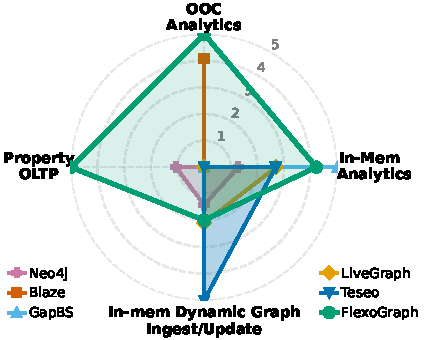
\includegraphics[scale=0.75]{fig/spider_chart_v2.pdf}
  \caption{\project{} delivers robust performance across the entire spectrum of operating conditions common in graph data management. Each axis represents a workload class; points closer to the boundary indicate better performance relative to the best system in that class.}
  \label{fig:fg-spider}
\end{figure}

\section{Dissertation Organization}
\label{sec:intro:organization}

The remainder of this dissertation is organized as follows.
\autoref{sec:bg} introduces core concepts that are necessary to understand the landscape of graph data management systems. 
We look at two graph data models that conceptualize the graph data, and the data structures can be used to represent graphs in memory and on disk.
The chapter takes a look at some strategies that can be used for handling data that is larger than installed memory. 
The chapter concludes with a brief introduction to the \wt{} storage engine and all the internal concepts that inspire the \project{} architecture and are critical to understanding performance.

\autoref{chap:design_space} surveys the graph data management landscape, classifies existing systems along axes of graph model, mutability, and transaction support, and identifies the design point that \project{} occupies.
Since \project{} can \emph{flexibly} operate under conditions that vary along these axes, it is important to look at some exemplar systems along several points in the space.
We particularly focus on the systems that we use to benchmark \project{}'s performance against.

\autoref{sec:architecture:structural} and \autoref{sec:architecture:property} present \project{}'s design in two parts.
The first describes how two complementary structural layouts are encoded in \wt{}'s B-tree, along with the cursor abstraction and partitioning strategies that enable parallel analytics.
The second introduces the label encoding scheme and two property storage modes, embedded and columnar, that decouple property storage from structural storage.

We evaluate \project{} across three workload classes that span four operating regimes. 
\autoref{sec:eval:static} compares \emph{static structural graph} analytics performance against in-memory and out-of-core systems.
\autoref{sec:eval:dynamic:chapter} measures insertion scalability and post-ingestion analytics on \emph{dynamic structural graphs} against other in-memory systems.
\autoref{sec:eval:property:chapter} evaluates \emph{property graph} workloads using the LDBC Social Network Benchmark against Neo4j, ArangoDB, and JanusGraph.

In \autoref{sec:future-work}, we explore three promising reseach projects that naturally follow the work presented in this dissertation: learned indexes on the property graph based on access pattern, integrating a high-level query language and identifying what query planning and optimization look like absent a cost model and traditional catalog, and supporting graph machine workloads in \project{}.
Finally, we conclude the dissertation in \autoref{sec:conclusion}, with a recap and synthesis of our contributions to the field of graph data management.